\documentclass[10pt,twocolumn]{article}
\usepackage[letterpaper,margin=1in]{geometry}
\usepackage{newtxtext,newtxmath}
\let\Bbbk\relax
\usepackage[utf8]{inputenc}
\usepackage[T1]{fontenc}
\usepackage{amsmath,amssymb,amsfonts}
\usepackage{booktabs}
\usepackage{graphicx}
\usepackage{hyperref}
\usepackage{cleveref}
\usepackage{microtype}
\usepackage[numbers,sort&compress]{natbib}
\usepackage{doi}
\usepackage{dblfloatfix}
\usepackage{algorithm}
\usepackage{algpseudocode}
\usepackage{enumitem}
\graphicspath{{figures/}{paper/en/figures/}{paper/fa/figures/}}
\usepackage{titlesec}
\setlength{\columnsep}{18pt}
\setlength{\emergencystretch}{2em}
\titleformat{\section}{\large\bfseries}{\thesection}{0.7em}{}
\titleformat{\subsection}{\normalsize\bfseries}{\thesubsection}{0.7em}{}
\titleformat{\subsubsection}{\normalsize\bfseries}{\thesubsubsection}{0.7em}{}
\titlespacing*{\section}{0pt}{1.0ex plus 0.3ex minus 0.2ex}{0.6ex}
\titlespacing*{\subsection}{0pt}{0.8ex plus 0.2ex minus 0.2ex}{0.4ex}
\titlespacing*{\subsubsection}{0pt}{0.6ex plus 0.2ex minus 0.1ex}{0.3ex}

\title{CF-MARLOS-AVA: Adaptive Vector-Aligned Federated Multi-Agent Reinforcement Learning for Open-Set Blockchain Intrusion Detection}
\author{Mohammad Hassan Amini\\{\small M.Sc. Student, Iran University of Science and Technology}\\{\small \texttt{m\_amini79@cmps2.iust.ac.ir}}}
\date{}
\newcommand{\keywords}[1]{\par\medskip\noindent\textbf{Keywords:} #1\par\medskip}

\hypersetup{
  pdftitle={CF-MARLOS-AVA: Adaptive Vector-Aligned Federated Multi-Agent Reinforcement Learning for Open-Set Blockchain Intrusion Detection},
  pdfauthor={Mohammad Hassan Amini},
  pdfkeywords={federated learning, intrusion detection, open-set recognition, EVT, Double DQN, blockchain traffic},
}

\begin{document}
\maketitle

\begin{abstract}
CF-MARLOS-AVA is a cooperative federated intrusion-detection framework for B-NAT blockchain traffic that couples local CVAE-DQN training, Double-DQN policy learning, generator-based reconstruction, EVT-based open-set rejection, and adaptive vector-aligned utility-aware client aggregation. The system is built for horizontal federated learning under non-IID client partitions, so raw data remain local while the server coordinates shared representation learning. FedAvg and FedProx are used as standard baselines, while FMRL-AVA provides a utility-aware two-phase aggregation strategy that prioritizes informative clients and aligns selected update vectors before aggregation. After federated training, class-conditional EVT tails are fitted on validation reconstruction errors to calibrate a global unknown-rejection threshold. The proposed formulation targets three goals at once: preserve known-class performance, improve robustness under heterogeneous clients, and reject unseen attacks without destabilizing the closed-set classifier.
\end{abstract}

\keywords{federated learning \and intrusion detection \and open-set recognition \and EVT \and Double DQN \and blockchain traffic}

\section{Introduction}
Blockchain-based traffic and other distributed networked environments produce data that are naturally siloed across nodes, organizations, or monitoring points. This makes centralized training inconvenient and often unrealistic. Federated learning provides a natural alternative, but standard aggregation rules such as FedAvg can degrade when local client distributions are highly non-IID. The problem becomes more difficult in intrusion detection, where the model must not only classify known attack categories but also reject previously unseen attacks.

The repository underlying this paper implements a cooperative federated multi-agent reinforcement learning pipeline that treats known-class intrusion detection as a CVAE-DQN problem and adds an EVT-based open-set rejection stage after training. The proposed system is built around four trainable blocks: a prior network, a recognition network, a main Q-network, and a generator. A local target Q-network is retained for Double-DQN stability but is not federated as a separate object. The server aggregates shared parameters using FedAvg, FedProx, or FMRL-AVA. Closed-set runs use the full label set, while open-set evaluation keeps \texttt{FoT} as the held-out unknown attack.

The main contributions are:
\begin{itemize}[leftmargin=*]
  \item a federated CVAE-DQN architecture for blockchain intrusion detection under non-IID client partitions;
  \item a generator-based reconstruction path that supports EVT open-set calibration;
  \item a vector-aligned utility-aware two-phase federated aggregation method, FMRL-AVA, for heterogeneous clients;
  \item a complete evaluation protocol covering closed-set accuracy, open-set rejection, federated stability, and efficiency.
\end{itemize}

\section{Related Work}
Federated learning was introduced as a communication-efficient alternative to centralized learning in distributed settings \citep{mcmahan2017}. FedProx extends this idea by adding a proximal penalty that limits client drift in heterogeneous networks \citep{li2020}. In parallel, Double DQN reduces overestimation in Q-learning by decoupling action selection from target evaluation \citep{hasselt2016}. For open-set and unknown-class recognition, prior work has shown that confidence-based rejection is often insufficient, motivating tail modeling and EVT-style calibration \citep{bendale2016,rudd2018}.

The present work also builds on two aggregation references. FMRL-LA introduced a cost-efficient federated MARL design with two-phase communication, asynchronous per-agent critics, and a centralized learnable aggregator for utility-aware selection \citep{zhang2024fmrl}. FedAWA introduced client-vector based aggregation, where local update directions guide adaptive server-side aggregation weights without proxy data \citep{shi2025fedawa}. CF-MARLOS-AVA combines these ideas but adapts them to intrusion detection: the utility input is built from CVAE-DQN audit signals, validation/support rewards train and monitor the critic-mixer instead of directly weighting aggregation, and Phase B uses bounded update-vector alignment so IID-like rounds remain close to FedAvg.

\section{Problem Formulation}
Let $\mathcal{D}_i = \{(x_j, y_j)\}$ denote the local dataset on client $i$, where $x_j$ is a traffic feature vector and $y_j$ is one of the known labels. The client set is $\{1,\dots,N\}$. The known-label set is
\[
\mathcal{Y}_k = \{\text{Normal}, \text{BP}, \text{DoS}, \text{MitM}\},
\]
while unseen attacks are mapped to an unknown label during evaluation.

The federated objective is to minimize the weighted sum of client losses:
\[
\min_{\theta}\; \sum_{i=1}^{N} \frac{n_i}{\sum_j n_j} F_i(\theta),
\]
where $n_i$ is the number of local samples on client $i$. Under FedProx, the local objective becomes
\[
F_i^{\mathrm{prox}}(\theta) = F_i(\theta) + \frac{\mu}{2}\lVert \theta - \theta^{k-1}\rVert_2^2.
\]
In FMRL-AVA, the server instead applies vector-aligned utility-weighted aggregation:
\[
\begin{aligned}
b_i &= n_i u_i,\\
\bar{\Delta} &= \frac{\sum_{j \in A_k} b_j(\theta_j^k - \theta^{k-1})}{\sum_{j \in A_k} b_j},\\
m_i &= \mathrm{clip}\!\left(\exp(\kappa \cos(\theta_i^k-\theta^{k-1}, \bar{\Delta})), m_{\min}, m_{\max}\right),\\
a_i &= b_i m_i,\\
\theta^{k} &= \theta^{k-1} + \eta \frac{\sum_{i \in A_k} a_i(\theta_i^k - \theta^{k-1})}{\sum_{i \in A_k} a_i},
\end{aligned}
\]
where $A_k$ is the selected client set, $u_i$ is the estimated utility of client $i$, and $m_i$ is a bounded update-vector alignment multiplier. The sample-count prior remains intact through $n_i$, while clients whose updates align better with the round reference direction receive more influence.

\section{Proposed Methodology}
We consider a horizontal federated setting in which each client trains locally on a private shard of B-NAT traffic. The server never receives raw samples. Instead, it receives model parameters and audit summaries, then performs aggregation and calibration in a controlled sequence. The full pipeline is illustrated in Figure~\ref{fig:overview}.

\subsection{System Overview}
The system begins with raw B-NAT CSV traffic, which is preprocessed into tensors and partitioned into non-IID client shards. Clients perform local CVAE-DQN training, the server aggregates the resulting updates, and a global model is calibrated on validation reconstruction errors through EVT. This yields a thresholded open-set classifier that can preserve known-class performance while rejecting unknown attacks.

\begin{figure*}[t]
  \centering
  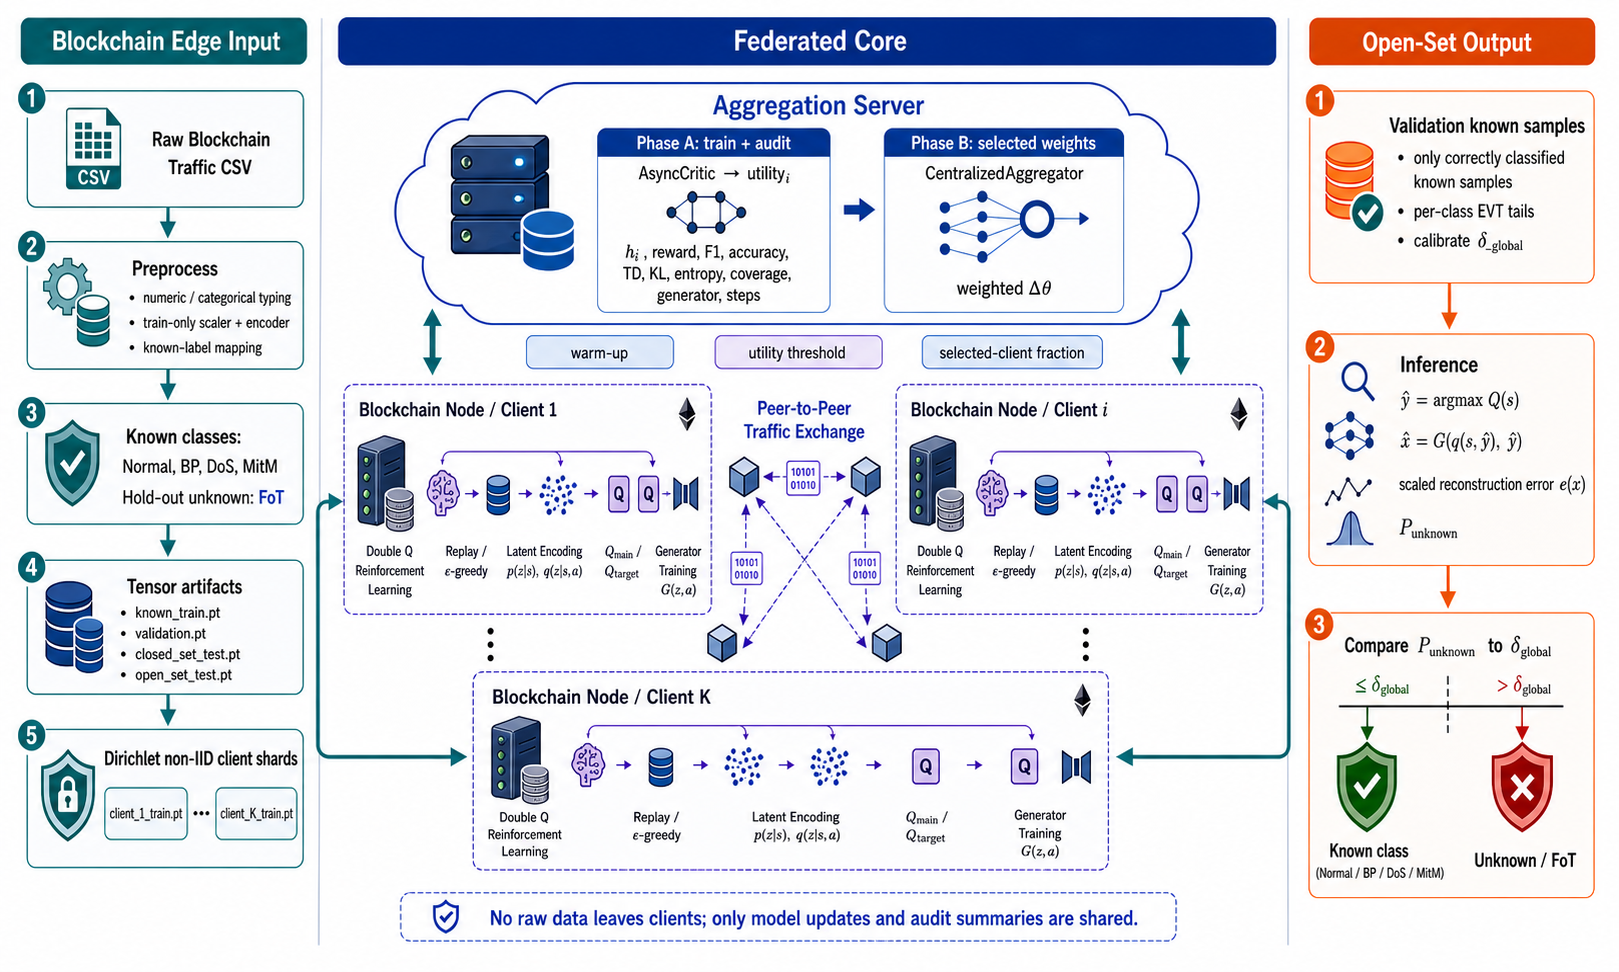
\includegraphics[width=\textwidth]{proposed_method_overview.png}
  \caption{Overview of CF-MARLOS-AVA: preprocessing, non-IID client shards, local CVAE-DQN training, federated aggregation, and EVT-based open-set inference.}
  \label{fig:overview}
\end{figure*}

\begin{algorithm}[t]
\caption{Federated CVAE-DQN Training and Open-Set Calibration}
\begin{algorithmic}[1]
\Require Client datasets $\{D_i\}_{i=1}^N$, validation set $D_{\mathrm{val}}$, rounds $K$, local configuration $H$, strategy $S \in \{\mathrm{FedAvg}, \mathrm{FedProx}, \mathrm{FMRL\text{-}AVA}\}$
\Ensure Final model $\theta^\ast$, EVT models $M_{\mathrm{evt}}$, rejection threshold $\delta$
\State Initialize $\theta^0 = \{\theta_p^0,\theta_r^0,\theta_Q^0,\theta_G^0\}$
\For{$k = 1$ to $K$}
  \State Server samples clients $C_k$ and broadcasts $\theta^{k-1}$
  \ForAll{$i \in C_k$ \textbf{in parallel}}
    \State $\mu_i \gets \mu$ if $S=\mathrm{FedProx}$ else $0$
    \State $(\theta_i^k, m_i^k) \gets \textsc{ClientLocalUpdate}(D_i,\theta^{k-1},H,\mu_i)$
  \EndFor
  \If{$S=\mathrm{FMRL\text{-}AVA}$}
    \State $\theta^k \gets \textsc{FMRLAVAUpdate}(\theta^{k-1},\{(\theta_i^k,m_i^k)\})$
  \Else
    \State $\theta^k \gets \frac{\sum_{i\in C_k} n_i \theta_i^k}{\sum_{i\in C_k} n_i}$
  \EndIf
\EndFor
\State $\theta^\ast \gets \theta^K$
\State $(M_{\mathrm{evt}}, \delta) \gets \textsc{EVTCalibration}(D_{\mathrm{val}}, \theta^\ast)$
\State \Return $\theta^\ast, M_{\mathrm{evt}}, \delta$
\end{algorithmic}
\end{algorithm}

\subsection{Local CVAE-DQN Agent}
Each client contains a CVAE-DQN agent with four learned components: a prior network $p_\theta(z|s)$, a recognition network $q_\phi(z|s,a)$, a main Q-network $Q_\psi(z,s)$, and a generator $G_\omega(z,a)$. A local target Q-network $Q_\psi^-$ is maintained only for temporal-difference stabilization. Replay memory and an epsilon-greedy policy support local interaction with the intrusion environment.

The local objective has three parts. The prior network is trained with a latent KL objective; the recognition and main Q-network are trained with a Double-DQN target; and, when FedProx is active, a proximal term constrains local drift from the broadcast global model. In compact form:
\[
L_{\mathrm{prior}} = \mathrm{KL}(q_\phi(z|s,a^\ast)\,\|\,p_\theta(z|s)),
\]
\[
y = r + \gamma(1-d)\,Q_\psi^{-}(z', s', \arg\max_a Q_\psi(z', s', a)),
\]
\[
L_{\mathrm{TD}} = \mathrm{Huber}(Q_\psi(z,s,a)-y),
\]
\[
L_{\mathrm{prox}} = \frac{\mu}{2}\lVert \theta - \theta^{k-1}\rVert_2^2.
\]

\begin{algorithm}[t]
\caption{Client-Side CVAE-DQN Local Update with Optional FedProx}
\begin{algorithmic}[1]
\Require Local data $D_i$, broadcast parameters $\theta^{k-1}$, local configuration $H$, proximal coefficient $\mu_i$
\Ensure Updated parameters $\theta_i^k$, diagnostics $m_i^k$
\State Load $\theta^{k-1}$ into $p_\theta$, $q_\phi$, $Q_\psi$, and $G_\omega$
\State Set $Q_\psi^- \gets Q_\psi$ and store $\theta^{k-1}$ as the proximal reference
\State Initialize replay buffer $B_i$ and epsilon-greedy policy $\pi_i$
\For{each local episode}
  \State Interact with the local environment and store transitions $(s_t,a_t,r_t,s_{t+1},d_t,a_t^\ast)$ in $B_i$
  \If{$|B_i|$ is sufficient}
    \State Sample a mini-batch from $B_i$
    \State Update $p_\theta$ using $L_{\mathrm{prior}}$ and, if active, the FedProx penalty
    \State Update $q_\phi$ and $Q_\psi$ using $L_{\mathrm{TD}}$ and, if active, the FedProx penalty
    \State Periodically soft-update or hard-copy $Q_\psi^-$ from $Q_\psi$
  \EndIf
\EndFor
\State Build the set of correctly classified known samples
\If{generator training is enabled}
  \State Train $G_\omega$ only on correctly classified known samples
\EndIf
\State \Return $\theta_i^k = \{\theta_p,\theta_r,\theta_Q,\theta_G\}$ and diagnostics $m_i^k$
\end{algorithmic}
\end{algorithm}

\subsection{Generator-Based Reconstruction}
The generator reconstructs an input feature vector from a latent code and a class condition:
\[
\hat{x} = G_\omega(z,a).
\]
It is trained only on correctly classified known samples so that the reconstruction error reflects the geometry of the known-class manifold rather than noise introduced by misclassified or unknown data. This error later becomes the basis for the open-set detector.

\subsection{Federated Parameter Sharing}
Only trainable parameters that define the shared representation are federated.

\begin{table}[t]
\centering
\caption{Federated and non-federated components}
\begin{tabular}{p{0.42\linewidth}p{0.48\linewidth}}
\toprule
\textbf{Federated} & \textbf{Role} \\
\midrule
Prior network $p_\theta(z|s)$ & Shared latent structure \\
Recognition network $q_\phi(z|s,a)$ & Latent inference and reconstruction \\
Main Q-network $Q_\psi(z,s)$ & Global known-class policy \\
Generator $G_\omega(z,a)$ & Shared reconstruction behavior \\
\midrule
\textbf{Not federated} & \textbf{Role} \\
\midrule
Target Q-network $Q_\psi^-$ & Local stabilization copy \\
Replay buffer & Local trajectory history \\
Optimizer state & Private training state \\
EVT models and thresholds & Post-training calibration artifacts \\
Raw client data & Remains local for privacy \\
\bottomrule
\end{tabular}
\end{table}

\subsection{FedAvg and FedProx Baselines}
FedAvg is the canonical baseline and uses sample-weighted averaging. FedProx keeps the same server aggregation rule but modifies the local objective with a proximal penalty. In this paper, FedAvg and FedProx are treated as baseline optimization strategies rather than separate algorithmic contributions.

\subsection{FMRL-AVA Cooperative Aggregation}
FMRL-AVA is the proposed cooperative aggregation mechanism. The name denotes \emph{Federated Multi-Agent Reinforcement Learning with Adaptive Vector-Aligned Aggregation}. It is not a direct reproduction of either source method: Phase A follows the FMRL-LA idea of two-phase communication, asynchronous critics, and utility-aware selection \citep{zhang2024fmrl}, while Phase B follows the FedAWA idea that client update vectors reveal useful information about local data heterogeneity \citep{shi2025fedawa}. In Phase A, clients train locally and upload audit metadata. The server estimates utility from latent summaries and diagnostics such as reward, accuracy, F1, TD stability, novelty, class entropy, label coverage, generator quality, and step count. In Phase B, selected clients upload cached weights and the server applies a bounded adaptive vector-aligned utility-weighted update.

\begin{algorithm}[t]
\caption{FMRL-AVA Vector-Aligned Utility-Aware Client Selection and Aggregation}
\begin{algorithmic}[1]
\Require Previous global parameters $\theta^{k-1}$, client updates and diagnostics $\{(\theta_i^k,m_i^k)\}$, utility threshold $\lambda$, minimum selected clients $q_{\min}$, maximum fraction $\rho_{\max}$, step size $\eta$, alignment strength $\kappa$, alignment bounds $[m_{\min},m_{\max}]$
\Ensure Updated global parameters $\theta^k$
\State Estimate utility $u_i$ for each client using latent summaries and diagnostics
\State Select $A_k = \{i : u_i \ge \lambda\}$
\If{$|A_k| < q_{\min}$}
  \State Add the highest-utility clients until $|A_k| = q_{\min}$
\EndIf
\State Limit $|A_k| \le \lceil \rho_{\max}|C_k| \rceil$
\ForAll{$i \in A_k$}
  \State $\Delta_i \gets \theta_i^k - \theta^{k-1}$
\EndFor
\State $b_i \gets n_i u_i$ for all $i \in A_k$
\State $\bar{\Delta} \gets \frac{\sum_{i \in A_k} b_i\Delta_i}{\sum_{i \in A_k} b_i}$
\ForAll{$i \in A_k$}
  \State $m_i \gets \mathrm{clip}(\exp(\kappa \cos(\Delta_i,\bar{\Delta})),m_{\min},m_{\max})$
  \State $a_i \gets b_i m_i$
\EndFor
\State $\theta^k \gets \theta^{k-1} + \eta \frac{\sum_{i \in A_k} a_i\Delta_i}{\sum_{i \in A_k} a_i}$
\State Update server-side critics and mixer using validation-aware monitoring targets
\State \Return $\theta^k$
\end{algorithmic}
\end{algorithm}

\subsection{EVT Open-Set Calibration}
After federated training, EVT is fitted on validation reconstruction errors that come only from correctly classified known samples. For each class, the upper tail of the reconstruction-error distribution is modeled with a generalized Pareto distribution. The resulting probability of unknownness is compared with a global threshold $\delta$.

\begin{algorithm}[t]
\caption{EVT Calibration and Open-Set Inference}
\begin{algorithmic}[1]
\Require Validation set $D_{\mathrm{val}}$, trained model $\theta^\ast$, tail fraction $\alpha_{\mathrm{evt}}$, target known false-positive rate $\beta$
\Ensure EVT models $M_{\mathrm{evt}}$, global threshold $\delta$, final prediction $\hat{y}$
\State Collect reconstruction errors for correctly classified known validation samples
\ForAll{known classes $c$}
  \State Fit an EVT tail model to the upper tail of the errors for class $c$
\EndFor
\State Estimate validation unknown probabilities and set $\delta$ from the $(1-\beta)$ quantile
\For{each inference sample $x$}
  \State Predict $\hat{c} = \arg\max_c Q_\psi(p_\theta(x),x,c)$
  \State Compute reconstruction error $e_x$ using $q_\phi$ and $G_\omega$
  \State Compute $p_u = M_{\mathrm{evt}}[\hat{c}](e_x)$
  \If{$p_u \ge \delta$}
    \State $\hat{y} \gets \text{Unknown}$
  \Else
    \State $\hat{y} \gets \hat{c}$
  \EndIf
\EndFor
\State \Return $M_{\mathrm{evt}}, \delta, \hat{y}$
\end{algorithmic}
\end{algorithm}

\subsection{Algorithmic Summary}
Algorithm~1 summarizes the end-to-end federated training and calibration flow. Algorithm~2 specifies the client-side CVAE-DQN update with the optional FedProx penalty. Algorithm~3 describes the utility-aware FMRL-AVA aggregation rule. Algorithm~4 closes the loop by fitting EVT on validation reconstruction errors and applying the open-set decision rule at inference time.

\section{Experimental Setup}
The evaluation protocol follows the repository contract and the experiment plan documented for the project. The primary dataset is B-NAT blockchain traffic. In the main B-NAT experiments, \texttt{Normal}, \texttt{BP}, \texttt{DoS}, and \texttt{MitM} are treated as known classes, while \texttt{FoT} is held out as the unknown attack. For the final manuscript, the primary configuration uses 10 clients and 100 logical federated rounds; smaller settings remain available in the repository for smoke tests and development runs.

All B-NAT comparisons reuse the same preprocessing contract, the same train/validation/test split, the same client partition seed, and the same evaluation seed list. Client shards are generated with Dirichlet non-IID sampling over class labels, with \(\alpha \in \{0.1, 0.5, 1.0, 10.0\}\) used to control skew. The main baselines are centralized training, local-only training, FedAvg, FedProx, and FMRL-AVA. Hydra controls the implementation details, including local episodes per round, replay-buffer size, batch size, Double-DQN settings, generator training, and open-set calibration toggles.

The external validation block is run independently on B-TAT, ToN-IoT, and CIC-IDS2017. Each dataset uses its own finalized known/unknown mapping, its own split, and its own non-IID partition; this block is therefore a separate validation study rather than a cross-dataset transfer experiment.

The reported protocol should be organized into eight experiments: closed-set validation, open-set detection, federated non-IID comparison, combined open-set plus non-IID evaluation, multi-dataset external validation, ablation and sensitivity, efficiency and scalability, and label-wise open-set stress testing. This structure follows the standard journal sequence of primary performance, robustness, external generalization, diagnostics, and efficiency.

\begin{table}[t]
\centering
\caption{Experimental matrix used in the final evaluation}
\begin{tabular}{p{0.14\linewidth}p{0.28\linewidth}p{0.42\linewidth}}
\toprule
\textbf{Exp.} & \textbf{Purpose} & \textbf{Primary output} \\
\midrule
E1 & Closed-set validation & Accuracy, macro F1, balanced accuracy \\
E2 & Open-set detection & AUROC, AUPRC, FPR@95\%TPR, unknown F1 \\
E3 & Non-IID federation & Stability, convergence, communication cost \\
E4 & Combined stress test & Known and unknown metrics under client skew \\
E5 & Multi-dataset external validation & Per-dataset accuracy, open-set metrics, and robustness under dataset-specific shifts \\
E6 & Ablation and sensitivity & Metric deltas and threshold robustness \\
E7 & Efficiency and scalability & Runtime, bytes transmitted, rounds to converge \\
E8 & Label-wise open-set test & Latent-space separation and per-label rejection \\
\bottomrule
\end{tabular}
\end{table}

\section{Evaluation Metrics}
Closed-set evaluation should report accuracy, macro precision, macro recall, macro F1, weighted F1, balanced accuracy, and per-class confusion matrices. These metrics quantify whether the model preserves ordinary known-class discrimination before any open-set rejection is applied.

Open-set evaluation should report AUROC, AUPRC, FPR@95\%TPR, TPR@5\%FPR, unknown F1, unknown rejection rate, and known accuracy after rejection. This combination is necessary because threshold-free and threshold-dependent metrics answer different questions: separability versus operational decision quality.

Federated evaluation should report final accuracy, final-10-round mean accuracy, convergence speed, client-wise variance, selected-client fraction, and communication cost. Efficiency should be reported through runtime, cumulative transmitted bytes, and accuracy per megabyte.

\section{Experimental Results and Discussion}
The results section should be organized around the eight experiments rather than around implementation details. E1 should verify that the core model preserves closed-set accuracy. E2 should isolate the value of EVT calibration for rejecting unknown attacks. E3 should compare FedAvg, FedProx, and FMRL-AVA under increasing client skew. E4 should combine both non-IID federation and open-set rejection to test system-level robustness. E5 should validate the method independently on B-TAT, ToN-IoT, and CIC-IDS2017 under separate dataset-specific known/unknown mappings and non-IID splits, without using B-NAT in that block. E6 should isolate the contribution of EVT, the generator, and utility-aware aggregation. E7 should quantify the cost of the two-phase federated mechanism. E8 should show whether open-set separation is consistent across held-out labels.

The discussion should explicitly interpret trade-offs. For example, if FMRL-AVA improves stability but increases coordination overhead, that trade-off should be shown with communication curves and round-wise accuracy plots. If EVT improves unknown rejection but slightly reduces known-class accuracy near the threshold, the calibration curve should make that effect visible.

\section{Ablation and Sensitivity}
The core ablations should remove EVT rejection, remove generator training, replace FMRL-AVA with FedAvg, replace FMRL-AVA with FedProx, and disable client selection by aggregating all uploaded models. Sensitivity analysis should sweep the EVT tail fraction, utility threshold, Dirichlet alpha, and random seeds. These results isolate the value of each module and show whether the method is robust to calibration choices.

\section{Limitations and Threats to Validity}
The main limitations are calibration sensitivity, the cost of two-phase federated coordination, and dataset-specific label mapping for the external benchmarks. EVT quality depends on validation splits, and FMRL-AVA requires additional server-side state and monitoring. These limitations should be acknowledged explicitly so the paper does not overstate generality.

\section{Reproducibility}
The repository provides Hydra-driven configuration, seed control, checkpointing, local artifact export, and run-level plots. These features make the pipeline reproducible across preprocessing, training, evaluation, and figure generation. The final manuscript should reference the stored outputs and fixed evaluation contract so that the reported results can be reproduced from the same split and seed list.

\section{Conclusion}
CF-MARLOS-AVA combines local CVAE-DQN learning, federated aggregation, generator-based reconstruction, and EVT open-set calibration into a single intrusion-detection framework. FedAvg and FedProx provide standard baselines, while FMRL-AVA adds vector-aligned utility-aware client selection for heterogeneous data. The resulting pipeline is designed to preserve known-class performance, reject unknown attacks, and remain stable under non-IID client partitions. The final experimental section should demonstrate these claims with matched budgets and controlled comparisons.

\begin{thebibliography}{99}
\bibitem{mcmahan2017}
H.~B. McMahan, E. Moore, D. Ramage, S. Hampson, and B.~A. y Arcas.
\newblock Communication-efficient learning of deep networks from decentralized data.
\newblock In \emph{Proceedings of AISTATS}, pages 1273--1282, 2017.

\bibitem{li2020}
T. Li, A.~K. Sahu, A. Talwalkar, and V. Smith.
\newblock Federated optimization in heterogeneous networks.
\newblock In \emph{Proceedings of MLSys}, 2020.

\bibitem{hasselt2016}
H. van Hasselt, A. Guez, and D. Silver.
\newblock Deep reinforcement learning with double Q-learning.
\newblock In \emph{Proceedings of AAAI}, 2016.

\bibitem{bendale2016}
A. Bendale and T.~E. Boult.
\newblock Towards open set deep networks.
\newblock In \emph{Proceedings of CVPR}, pages 1563--1572, 2016.

\bibitem{rudd2018}
E.~M. Rudd, L.~P. Jain, W.~J. Scheirer, and T.~E. Boult.
\newblock The extreme value machine.
\newblock \emph{IEEE Transactions on Pattern Analysis and Machine Intelligence}, 40(3):762--768, 2018.

\bibitem{zhang2024fmrl}
Y. Zhang, S. Wang, Z. Chen, X. Xu, S. Funiak, and J. Liu.
\newblock Towards cost-efficient federated multi-agent RL with learnable aggregation.
\newblock In \emph{Proceedings of PAKDD}, Lecture Notes in Artificial Intelligence 14646, pages 171--183, 2024.
\newblock \doi{10.1007/978-981-97-2253-2_14}.

\bibitem{shi2025fedawa}
C. Shi, H. Zhao, B. Zhang, M. Zhou, D. Guo, and Y. Chang.
\newblock FedAWA: Adaptive optimization of aggregation weights in federated learning using client vectors.
\newblock In \emph{Proceedings of CVPR}, pages 30651--30660, 2025.
\end{thebibliography}

\end{document}
